\section{Introduction}

\begin{figure}[H]
    \centering
    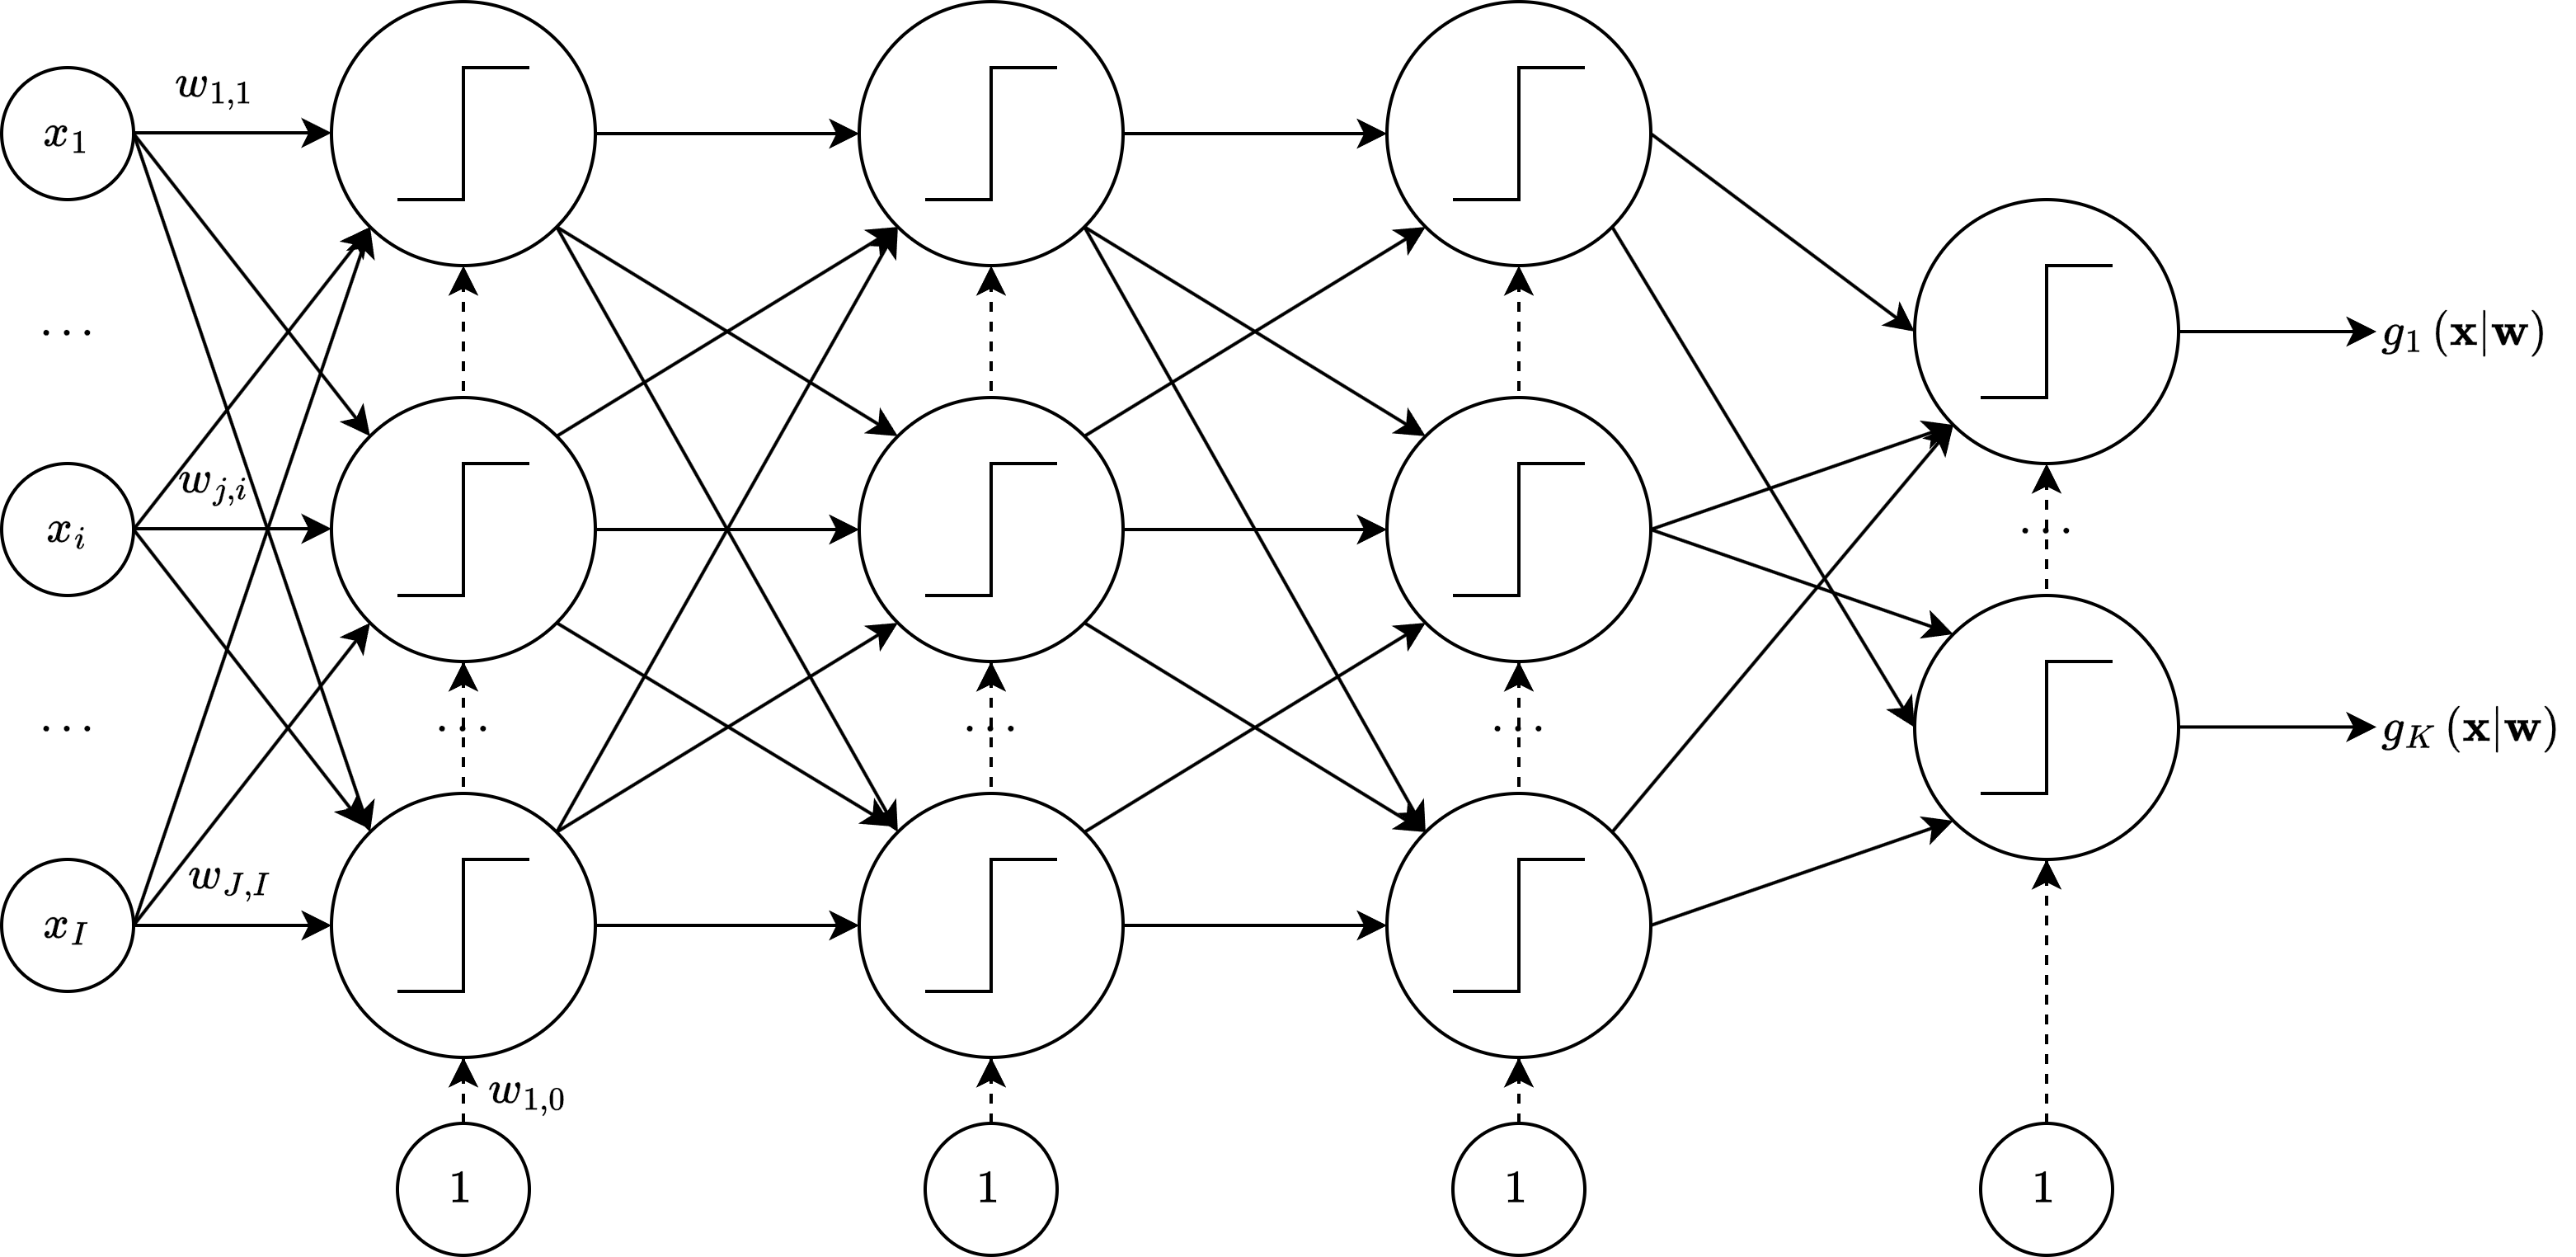
\includegraphics[width=0.75\linewidth]{images/ffnn.png}
    \caption{Multi-Layer Perceptron architecture}
\end{figure}
A Multi-Layer Perceptron is a type of Feed Forward Neural Network designed to process input data through multiple layers of interconnected nodes.
Each layer is Fully Connected to the next, forming a structure capable of learning complex relationships in data.
The Multi-Layer Perceptron architecture is organized into three main components:
\begin{itemize}
    \item \textit{Input layer}: this layer receives the raw input data and serves as the starting point for the network. 
        The size of the input layer corresponds to the number of input features, which varies depending on the specific problem being addressed.
    \item \textit{Hidden layers}: these intermediate layers are responsible for transforming the input data into more abstract representations.
        The number of hidden layers and the neurons within each layer are critical hyperparameters, typically determined through experimentation or optimization techniques.
    \item \textit{Output layer}: this final layer generates the network's output.
        The size of the output layer depends on the task at hand.
\end{itemize}
Multi-Layer Perceptrons are inherently non-linear models, characterized by their use of activation functions, the number of neurons in each layer, and the values of the connection weights.
The connections between layers are represented by weight matrices, where the weights determine the strength of the influence between neurons. 
The output of each neuron in the network depends solely on the outputs from the preceding layer, facilitating a forward propagation of information.